\subsubsection*{Creating the \acrshort{ast}}

The Class \texttt{VisitorAST} creates the \acrshort{ast} from the parse tree, it traverses the tree using the visitor pattern and on every node sets a field of a class in the \acrshort{ast}. 
Afterwards the node is placed on the tree as a leaf or a field on the node which made the visit call.

One of these visit methods can be seen on \myref{lst:VisitorASTCode}.

\begin{lstlisting}[caption=The Visit Method for WhileLoopNode,frame=tlrb,label={lst:VisitorASTCode}]
public BaseASTNode visitWhileLoop(ourLangParser.WhileLoopContext ctx) {
    WhileLoopNode whileLoopNode = new WhileLoopNode(parentStack.peek());
    whileLoopNode.setCondNode(
    	(ConditionalExpressionNode)visit(ctx.conditionalExpression()));
    parentStack.push(whileLoopNode);
    visitChildren(ctx.whileBlock);
    parentStack.pop();
    whileLoopNode.setLineNumber(ctx.start.getLine());
    return whileLoopNode;
}
\end{lstlisting}
A stack called the parentstack is used to keep track of the caller to \texttt{visit()}, in order to keep track of the parents and the children of the tree.
On lines three and four a call to visit the conditionalexpression of the whileloop is made, which returns an instance of the class \texttt{ConditionalExpressionNode}.
Afterwards, to set the body of the \texttt{WhileLoopNode}, all the children of the nodes are visited, but first the \texttt{WhileLoopNode} is pushed to the parentstack.
This makes it possible to check which node is the parent of the children being created during the calls to visit.

While implementing the Visitor pattern for the \acrshort{ast} an interface was made, which contains a visit method for every single class of the \acrshort{ast}.
A baseclass was then been made which implements this interface.
The baseclass implements each visit method such that the correct fields of the nodes are visited in the correct order.
This means that any visitor class only has to override the visit methods which are of interest for the specific visitor.
An UML diagram for the implementations of the visitor pattern in the compiler and can be seen on \myref{image:Visitors}.
The figure shows how every visitor class inherits from the \texttt{BaseASTVisitor} class.

\begin{figure}[!ht]
\centering
 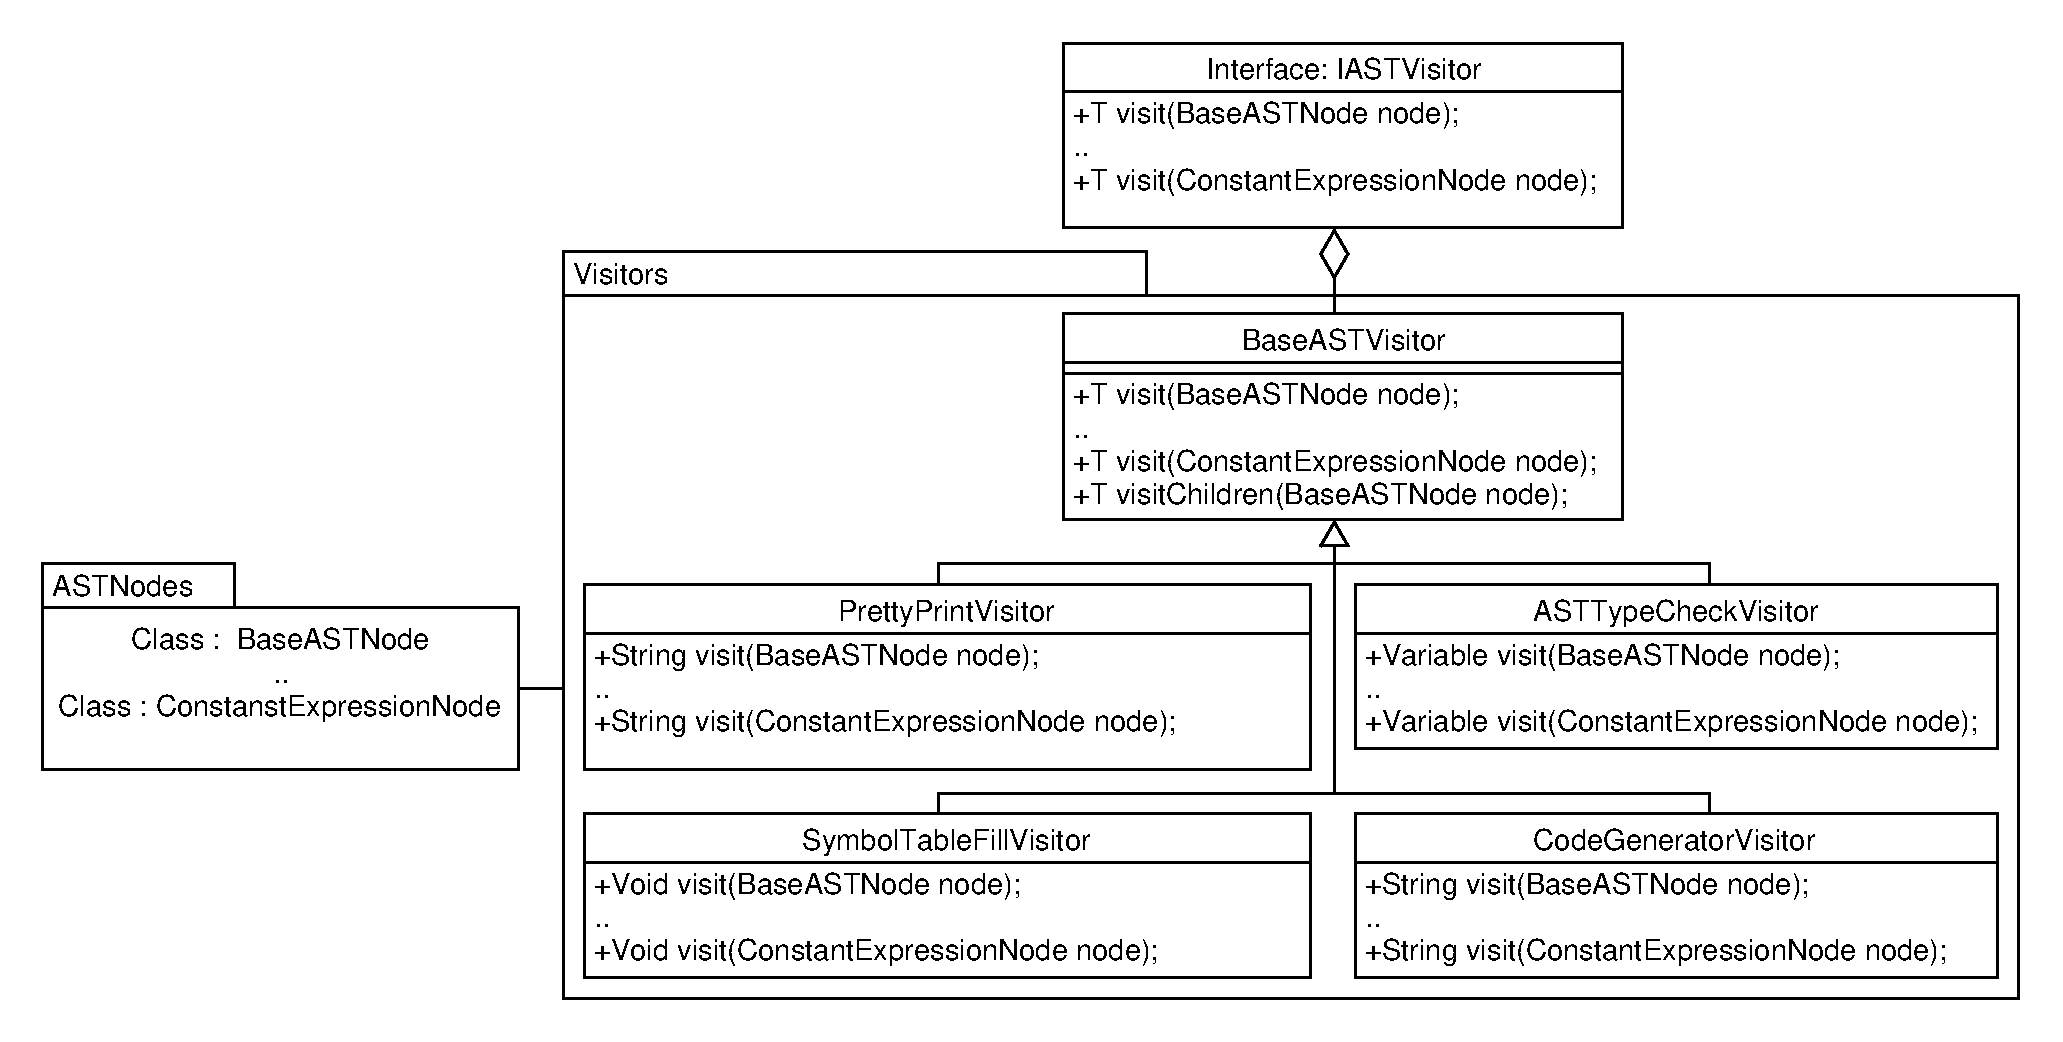
\includegraphics[width=1\textwidth]{figures/ClassDiagrams/Visitors.pdf} % trim=4.85cm 15cm 0.85cm 1cm
\caption{A UML diagram of the visitor patterns implementation in the compiler for traversing the \acrshort{ast}.}\label{image:Visitors}
\vspace{-15pt}
\end{figure} 